\section{Using functions with equal numbers of parameters} % 5 pages
\label{sec:functions}

The simplest application of the envelope method is to the case where all
functions used have the same number of parameters. This avoids several extra
complications which are discussed in Section~\ref{sec:correction}.
~\ref{sec:correction}
\subsection{Function definitions}
\label{sec:functions:function}

The first study presented uses four functions, each of which has two parameters.
These functions are chosen as they, and their higher order equivalents,
are feasible representations of the background shape seen in the Higgs to two photon
analysis. The functions are detailed below; in each case $p_0$ and $p_1$ are
the two parameters.
\begin{enumerate}
\item
``Power law''; $f(x) = p_0 x^{p_1}$.
\item
``Exponential''; $f(x) = p_0 e^{p_1x}$.
\item
``Laurent''; $f(x) = p_0/x^4 + p_1/x^5$.
\item
``Polynomial''; $f(x) = p_0 + p_1 x$.
\end{enumerate}

\subsection{Example case}
\label{sec:functions:example}

In the CMS Higgs to two photons analysis, the discrete profiling method is applied to
the actual data taken by the CMS experiment. The likelihood fit
is performed on the diphoton invariant mass spectrum simultaneously
across different event categories.
However, for the purposes of this
paper, the ``data'' used to illustrate the method are generated by a Monte Carlo
method from a smooth background
function which is similar in shape and magnitude to the
real data sample used. (However, it should be emphasised that this is not the
actual data sample and so
none of the detailed results presented below can be used to deduce any
properties of the Higgs boson itself.)
This dataset was generated in 160 bins between 110 and 150\,GeV in
the mass variable, $m_{\gamma\gamma}$.
It included signal events
generated according to a Gaussian distribution with a normalization of 50.8 events, a mean of 125\,GeV and a
width of 1.19\,GeV. These values are representative of the expected Higgs signal from a single category of the
CMS Higgs to two photons analysis.
In the following, the signal strength results are given in
terms of the relative strength $\mu$,
meaning the ratio of the measured number of the signal events relative
to the expected number.

The four two-parameter functions mentioned above were each
separately fitted to this
original dataset. A Gaussian signal component was also included, where the
mean and width of the Gaussian were fixed to the same values as used to
generate the events.
The magnitude of the signal Gaussian and both parameters in the
background function were determined from the fit.
The results are shown in figure~\ref{fig:functions:bestfits}.
It is clear the first order polynomial does not fit particularly well,
while the other three functions appear to give reasonable fits.
%
\begin{figure}[tbp]
\centering
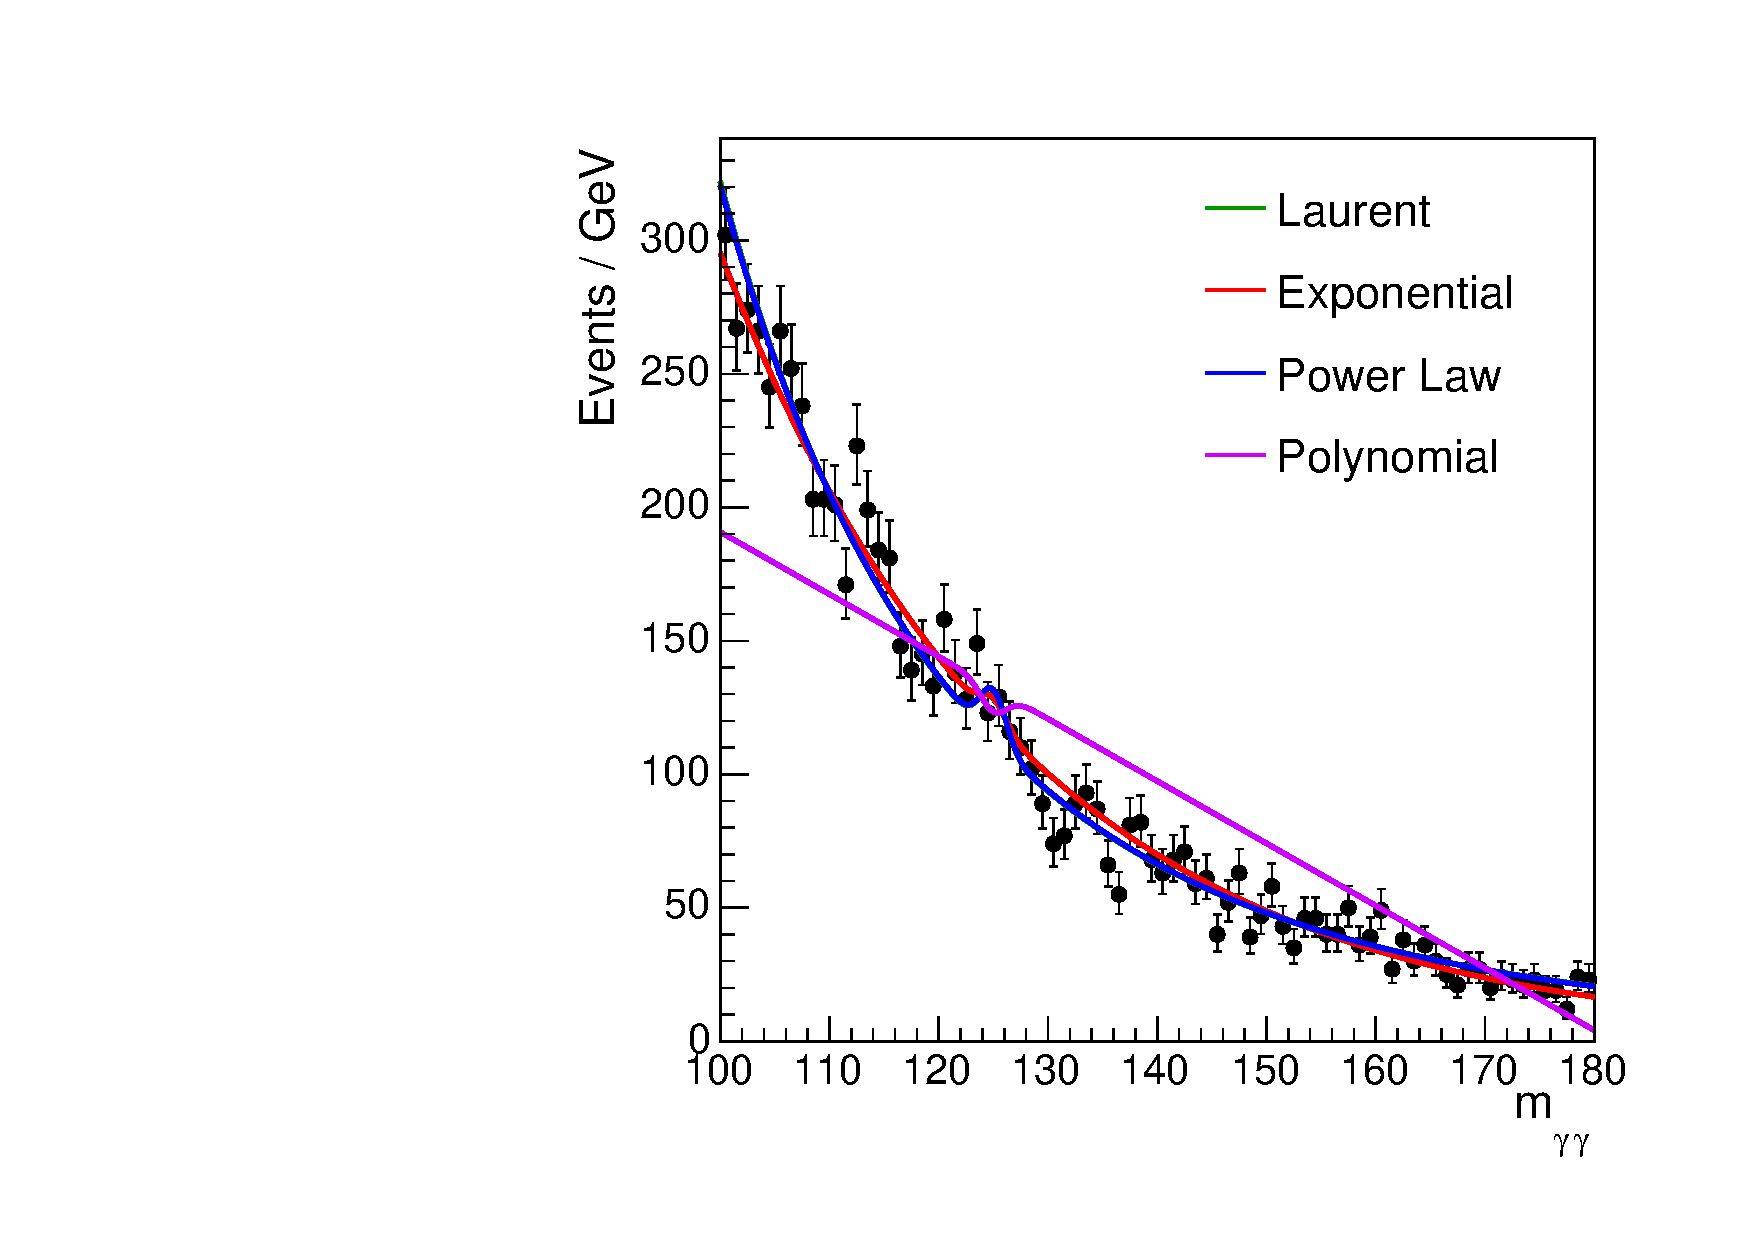
\includegraphics[width=0.45\textwidth]{functions/BestFits.pdf}
\caption{Best fits of the four two-parameter functions (described in the
text).
%The dashed lines indicate the background component of the fit while the solid
%lines include the signal component.
The Laurent function is effectively identical to the power law function
and so is hidden underneath the power law line.
Note, for clarity in this plot, the
data have been rebinned into 40 bins, although the fits were done with
finer binning of 160 bins.}
\label{fig:functions:bestfits}
\end{figure}

The profile scan as a function of the relative signal strength $\mu$
between $-1.0$ and 2.5
for the four functions is shown in
figure~\ref{fig:functions:profiles}.
The absolute minimum occurs for the power law function at a relative signal
strength of $\mu = 0.93$. When just considering this function,
the 68.3\% confidence interval on $\mu$ is
$0.43 < \mu < 1.40 $, determined as the interval for which $\Delta{\rm \nll} = \nll - \nll_{BF} < 1$.
The measurement would therefore be reported with its standard error as $\mu=0.93^{+0.47}_{-0.50}$. The Laurent function gives an identical result within the precision given.
When considering the exponential function alone, a slightly higher
\nll value is obtained
at the best fit point, which corresponds to a relative signal strength of $\mu = 0.72$
and a 68.3\% confidence interval of
$0.27 < \mu < 1.24 $, equivalently written as $\mu = 0.72^{+0.52}_{-0.45}$.
Fitting with the straight line yields a very different result of
$\mu = 0.01^{+0.51}_{-0.47}$
although it is clear that this function does not describe the data well and it
gives a much larger \nll value.
The fact that the different functions can give different best fit values
is a direct example of the systematic uncertainty associated
with the choice of function.
%
\begin{figure}[tbp]
\centering
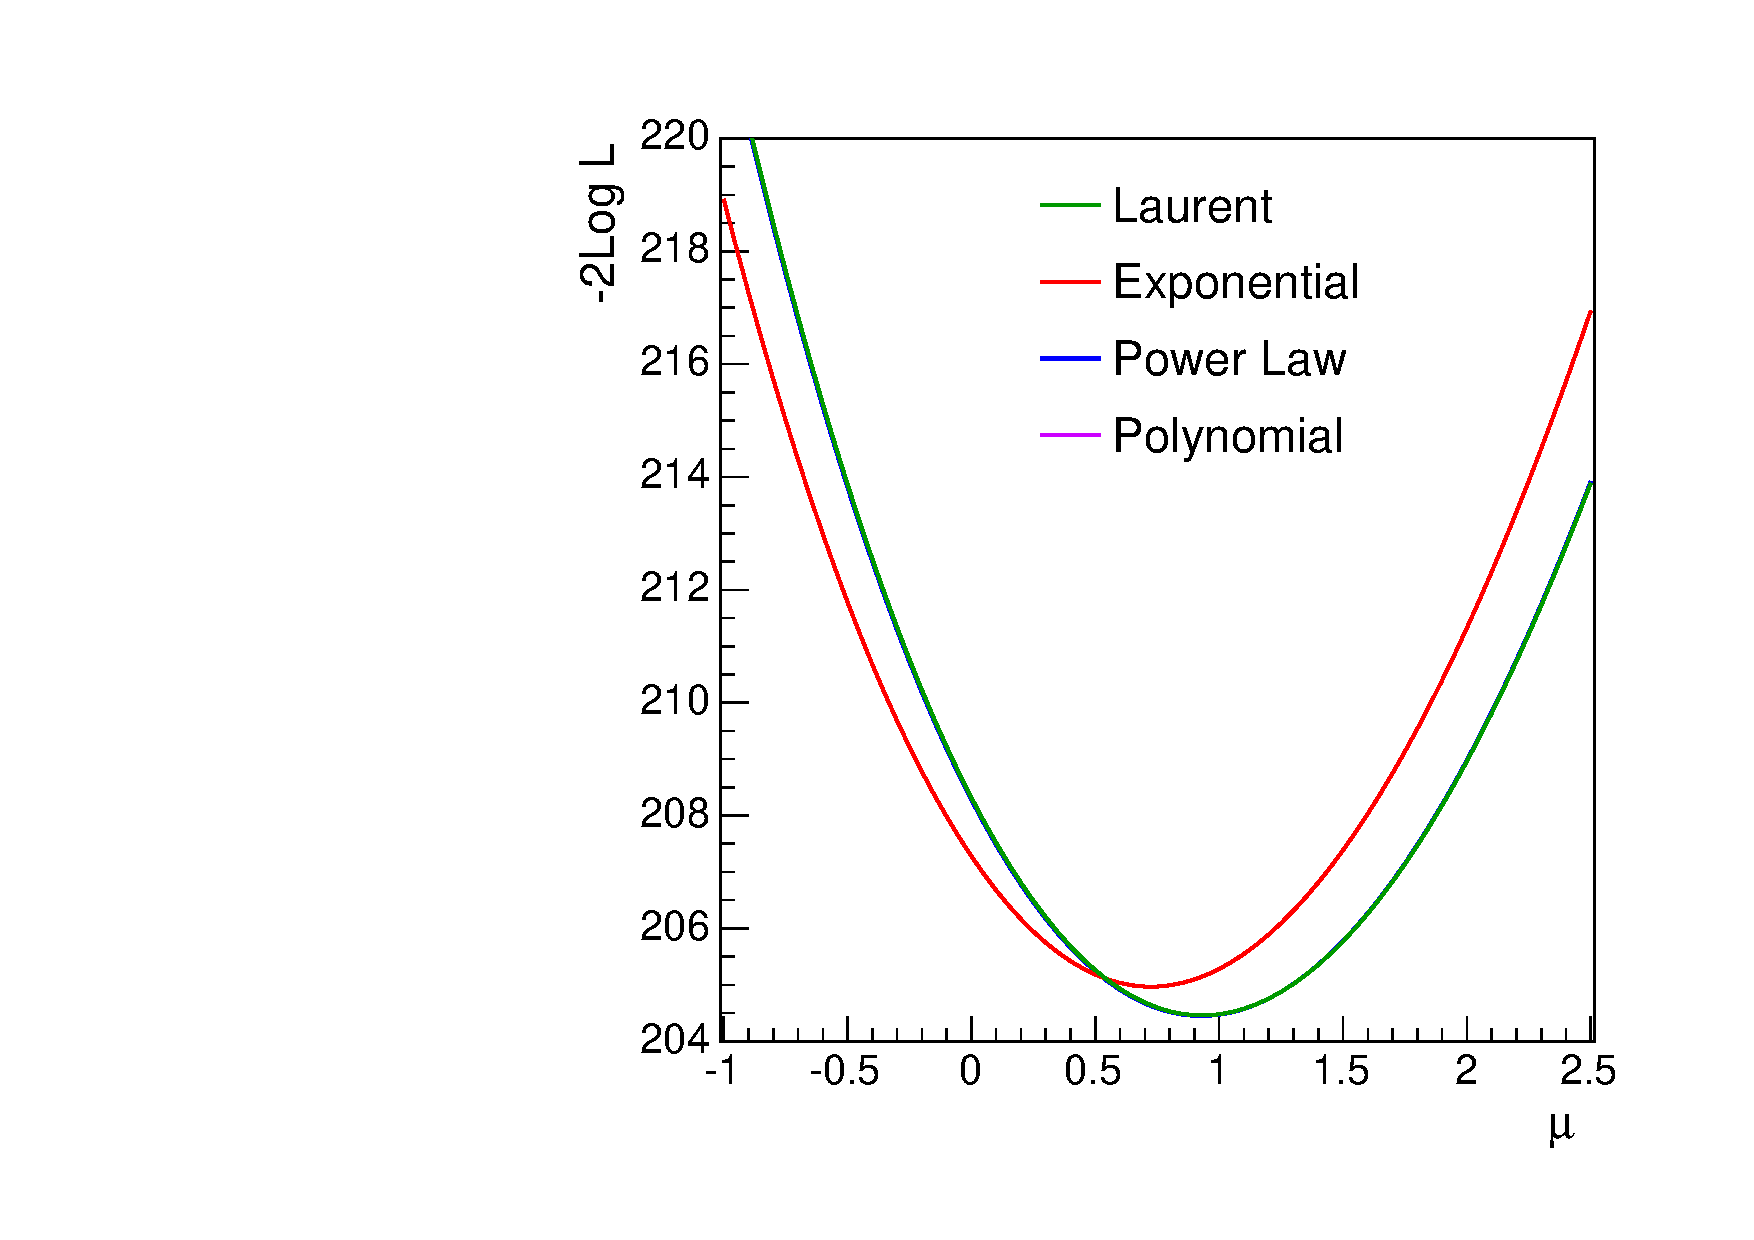
\includegraphics[width=0.45\textwidth]{functions/Profiles.pdf}
\caption{Profile \nll scans for the four two-parameter
functions discussed in the text.
The polynominal function is above the top of the \nll scale for all
$\mu$ values shown in this figure. }
\label{fig:functions:profiles}
\end{figure}

The envelope around these functions is shown in
figure~\ref{fig:functions:envelope}.
As it has to be, the best fit is still $\mu=0.93$ from the power law
but now the standard error is enlarged by the exponential function
contribution to the
envelope on the lower side of the scan. Hence, taking all four functions into
account, the 68.3\% confidence interval on $\mu$ is
$0.37 < \mu < 1.40 $, i.e. the lower limit extended by
the exponential fit and the upper limit from the power law fit.
The measured value of $\mu$ would now be quoted is
$\mu = 0.93_{-0.56}^{+0.47}$.
The enlarged uncertainty is a direct reflection of the
systematic error arising from the function uncertainty.
As also shown in figure~\ref{fig:functions:envelope}, the 95.4\% confidence
interval is $-0.18 < \mu < 1.92$.
There are two things to note. Firstly, although the Laurent fit
is effectively identical to the power law, there is no issue with
``double-counting'' as the envelope just takes the lowest \nll.
Also, it is clear that the poor fit of the polynomial
means it plays no role in the envelope and so this function is
``automatically'' ignored by the method,
without requiring any arbitrary criterion for
including it or not.
%
\begin{figure}[tbp]
\centering
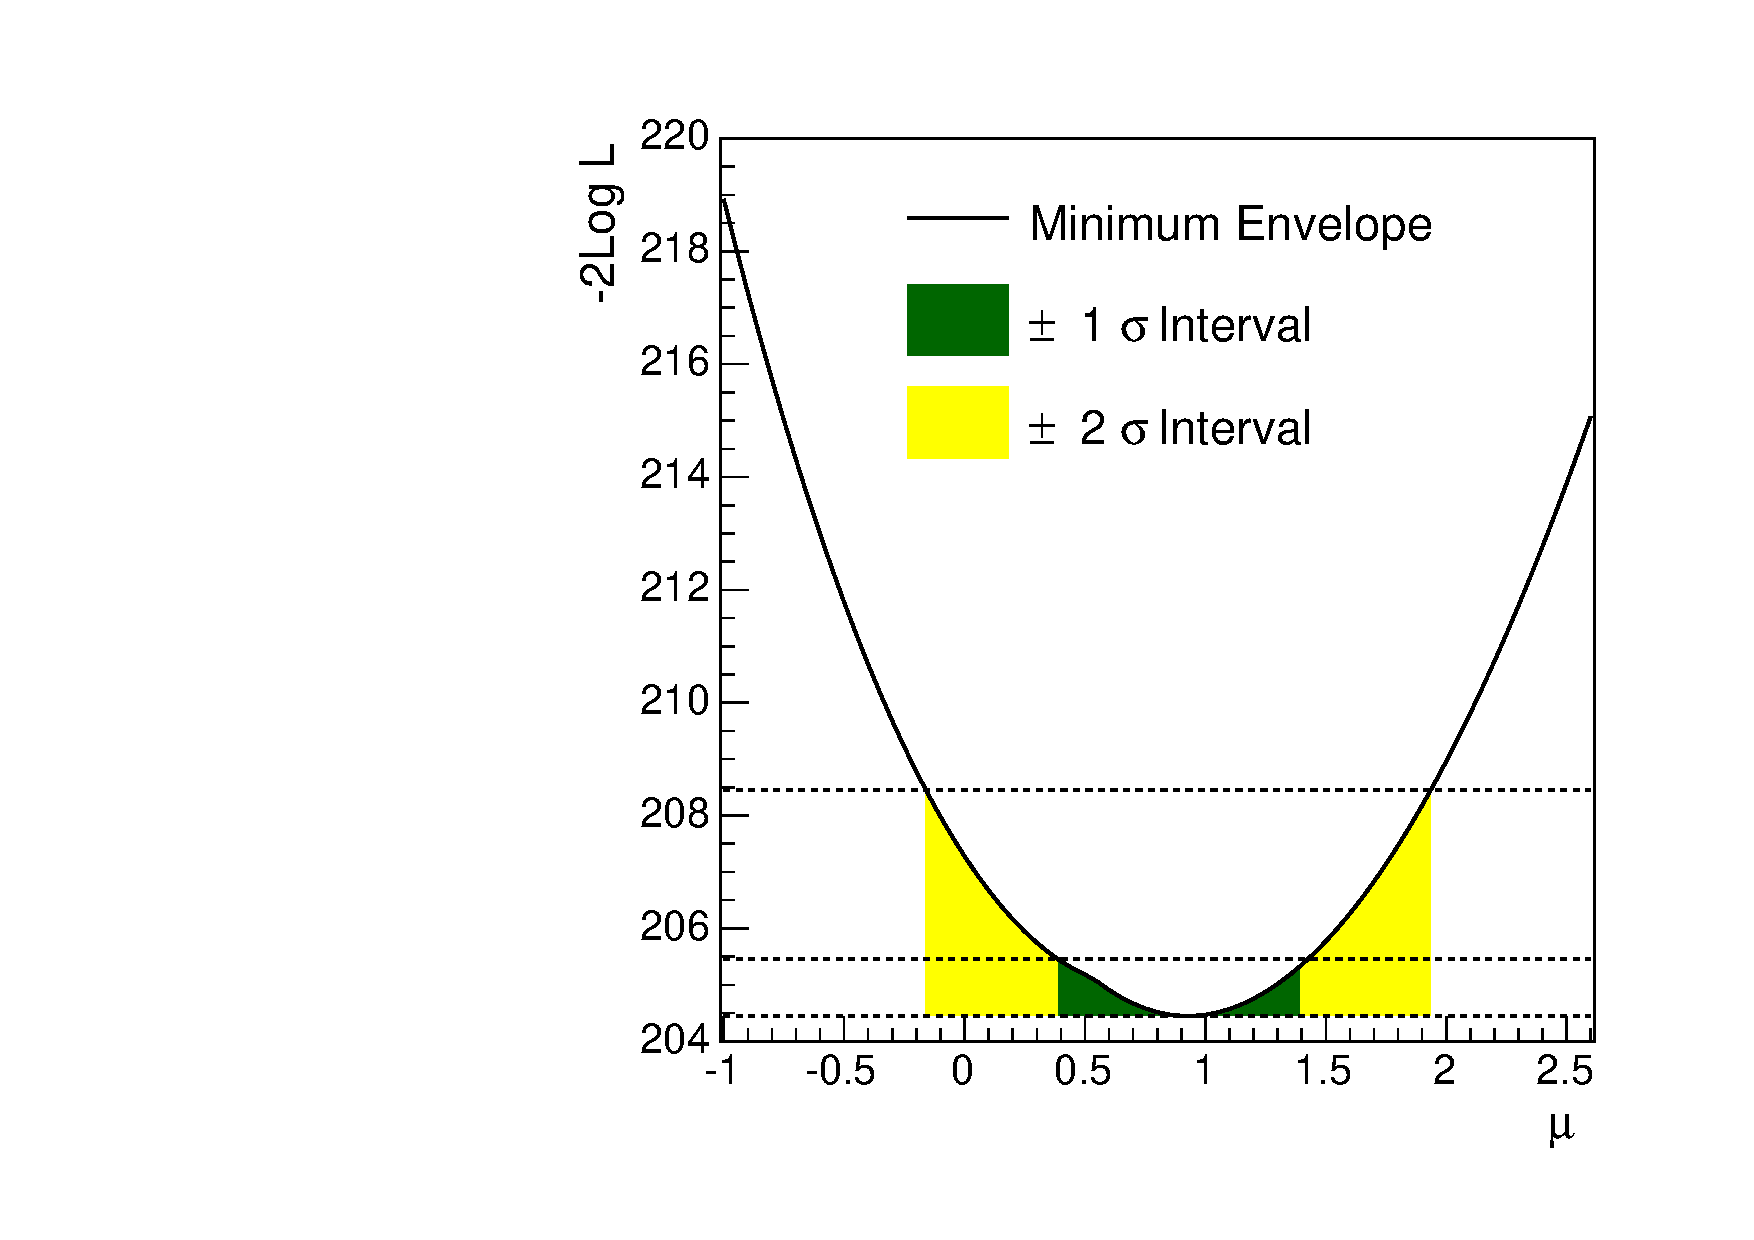
\includegraphics[width=0.45\textwidth]{functions/Envelope.pdf}
\caption{Profile \nll envelope for the four two-parameter function fits.
The coloured bands indicate the 68.3\% and 95.4\% intervals determined from the regions
for which the value of \nll increases by 1 and 4 units from the minimum value as indicated by the horizontal lines. The dashed red line shows the profile \nll
curve which would be obtained using just the power law function.}
\label{fig:functions:envelope}
\end{figure}


\subsection{Bias and coverage}
\label{sec:functions:coverage}

The bias and coverage properties of this method were tested
using a large ensemble of
pseudo-experiments (``toys''). In each pseudo-experiment, a
dataset including signal and background events was generated using a Monte Carlo technique.
Ensembles were generated, and consequently the bias and coverage properties tested, under various different background hypotheses and for different values of the signal strength, $\mu$. The background function from which the Monte Carlo events where generated was chosen to be one of the power law,
exponential or Laurent two-parameter functions discussed above in
section~\ref{sec:functions:function}. The background parameters for generating the toys are set to their best fit values for the given value of $\mu$.

In addition, a further ensemble of toy datasets was generated, for which the background function itself, as well
as its parameters, was chosen according to the best fit (i.e.~the minimum of the envelope) for each value of $\mu$. This is the background parametrisation which results from treating the choice of function as a discrete nuisance parameter. As can be seen from
figure~\ref{fig:functions:envelope}, this means that for values of $\mu < 0.55$ the exponential background
function will be used and it will be a power law function otherwise.
Conceptually, this method again
treats the choice of function as a discrete nuisance parameter and so picks the
best fit values of {\em all\/} nuisance parameters for each $\mu$ value.

The resulting toy datasets are now treated identically to the original dataset. The bias and coverage are assessed by calculating the fitted signal strength, $\mu$, and its error, $\sigma$, for each toy when using different background models. We define the bias as the mean of the pull distribution, where the pull for an individual toy is defined as
\begin{equation}
	p(\mu,\sigma) = \frac{\hat{\mu}-\mu}{\sigma},
\end{equation}
where $\mu$ is the generated value of the signal strength, $\hat{\mu}$ is the fitted value of $\mu$ per toy and $\sigma$ is the positive error on $\hat{\mu}$ if $\hat{\mu} < \mu$ and is the negative error on $\hat{\mu}$ if $\hat{\mu} > \mu$. The results of the mean pull as a function of the generated signal strength are shown in figure~\ref{fig:functions:firstorderbias}. It can be seen, as one would expect, that when fitting back with the same background function as used to generate the toy dataset, the bias is negligible. It is also shown that the bias is not dependent on the value of $\mu$ used to generate the signal. However, when fitting back with a different background function the bias can be large; here giving a mean pull up to 0.5.
The discrete profiling method provides a medium between these two in which the bias is small (a mean pull of around 0.1) regardless of the generating function used. This is important given that this method is to be applied when the true underlying function is unknown.

%
\begin{figure}[tbp]
\centering
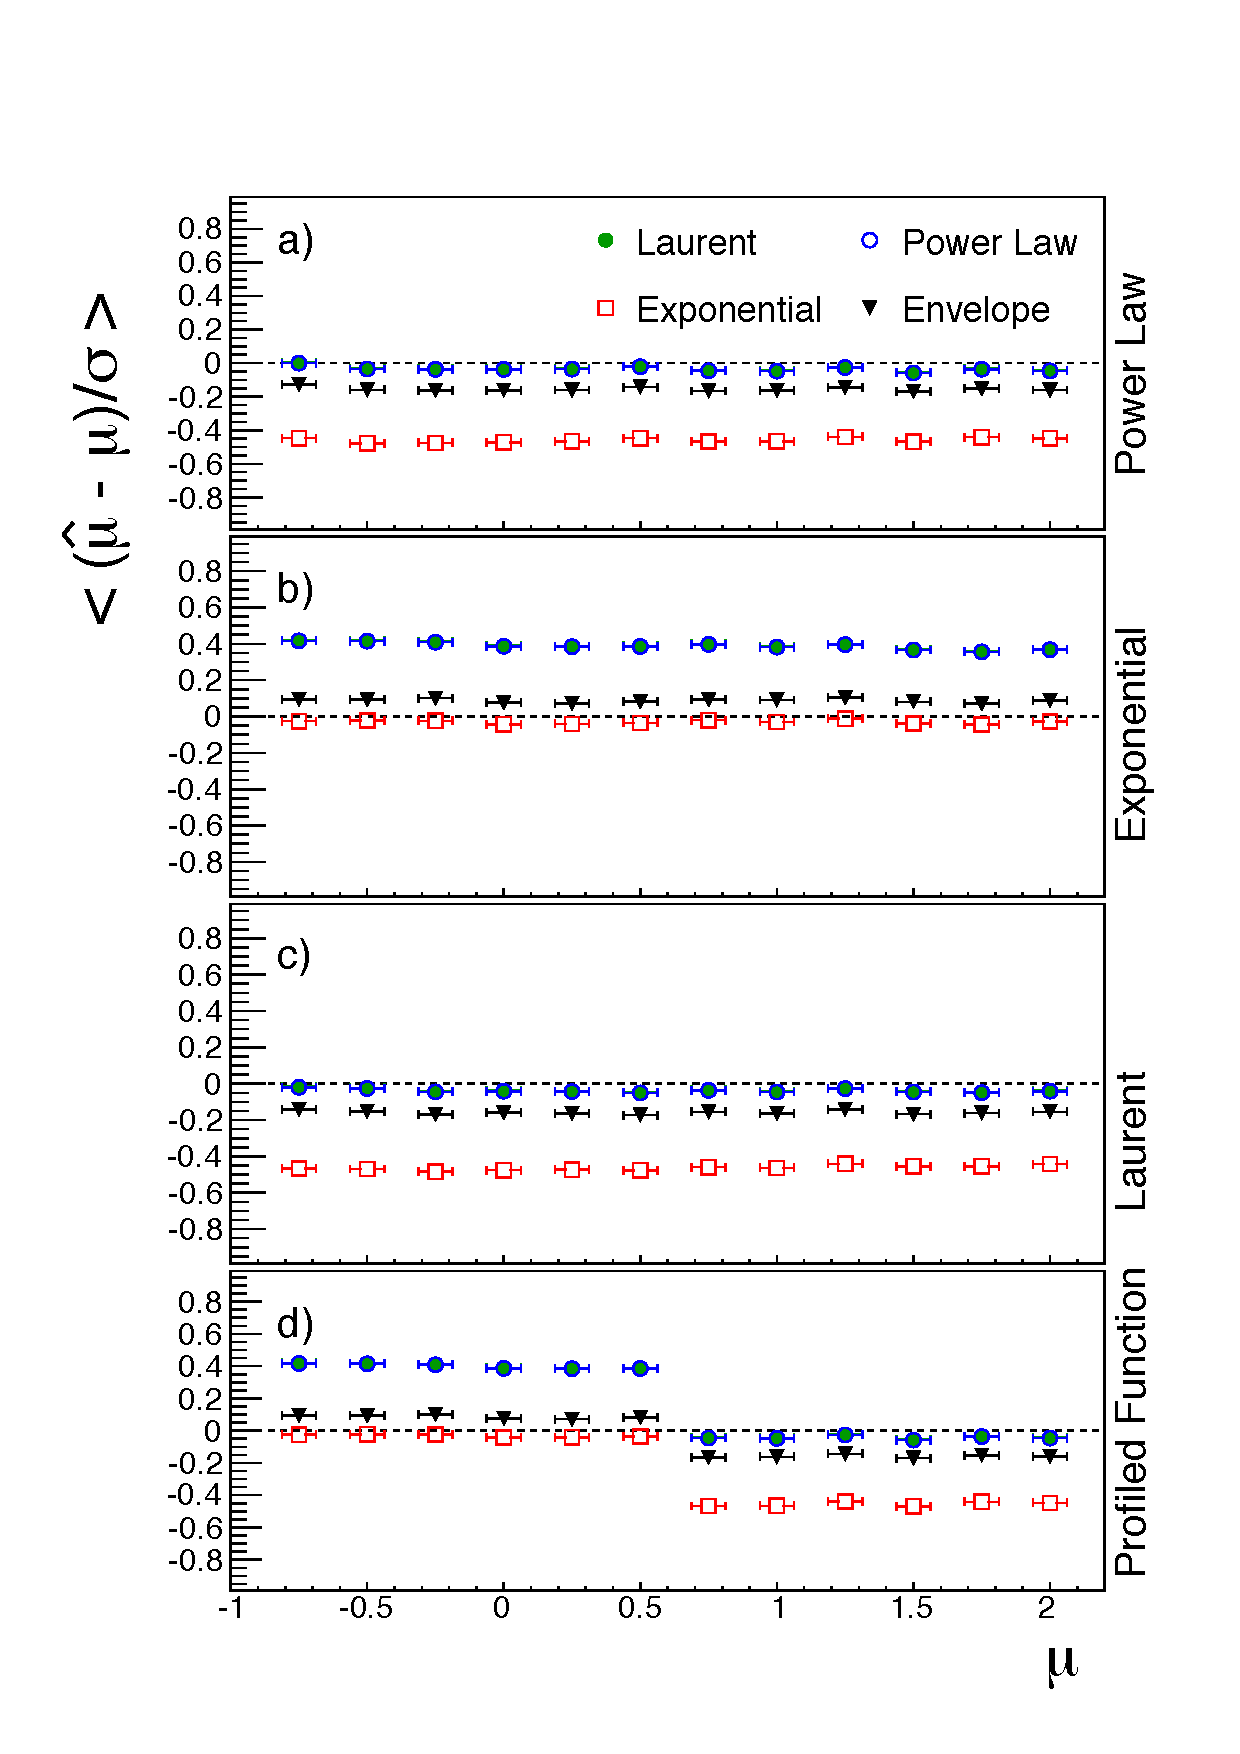
\includegraphics[width=0.48\textwidth]{functions/FirstOrderFunctions.pdf}
\caption{Average pull when fitting with each function as background and when
using the discrete profiling method. The first, second and third panels show the results
when the generating background function is power law, exponential and Laurent,
respectively. The last plot shows the result when the best-fit function at each
value of $\mu$ is used to generate toys; this means the exponential function
below $\mu = 0.55$ and the power law function above this value. Within each panel the different
points correspond to a different fitting function: Laurent (solid green), power law (open blue), exponential (open red) and the envelope of all four two-parameter functions (solid black). In all cases,
fitting with the polynomial gives values outside the range of these plots.}
\label{fig:functions:firstorderbias}
\end{figure}

The coverage was tested, using the same fits, by determining the frequency of toys in which the difference in \nll between the best fit value of $\mu$ and the value of $\mu$ used to generate the signal was less than 0.25, 1, 4 and 9.
These frequencies were compared with the expected frequencies, 38.3\%, 68.3\%, 95.4\% and 99.7\% respectively. The results for these are shown in figure~\ref{fig:functions:firstordercoverage}. It can be seen that when the fitting function is different from the generating function the calculated confidence interval can undercover, whereas when using the discrete profiling method the coverage is good regardless of the generating function. The coverage is found to be good,
independent of the value of $\mu$ used to generate the signal.
%
\begin{figure}[tbp]
\centering
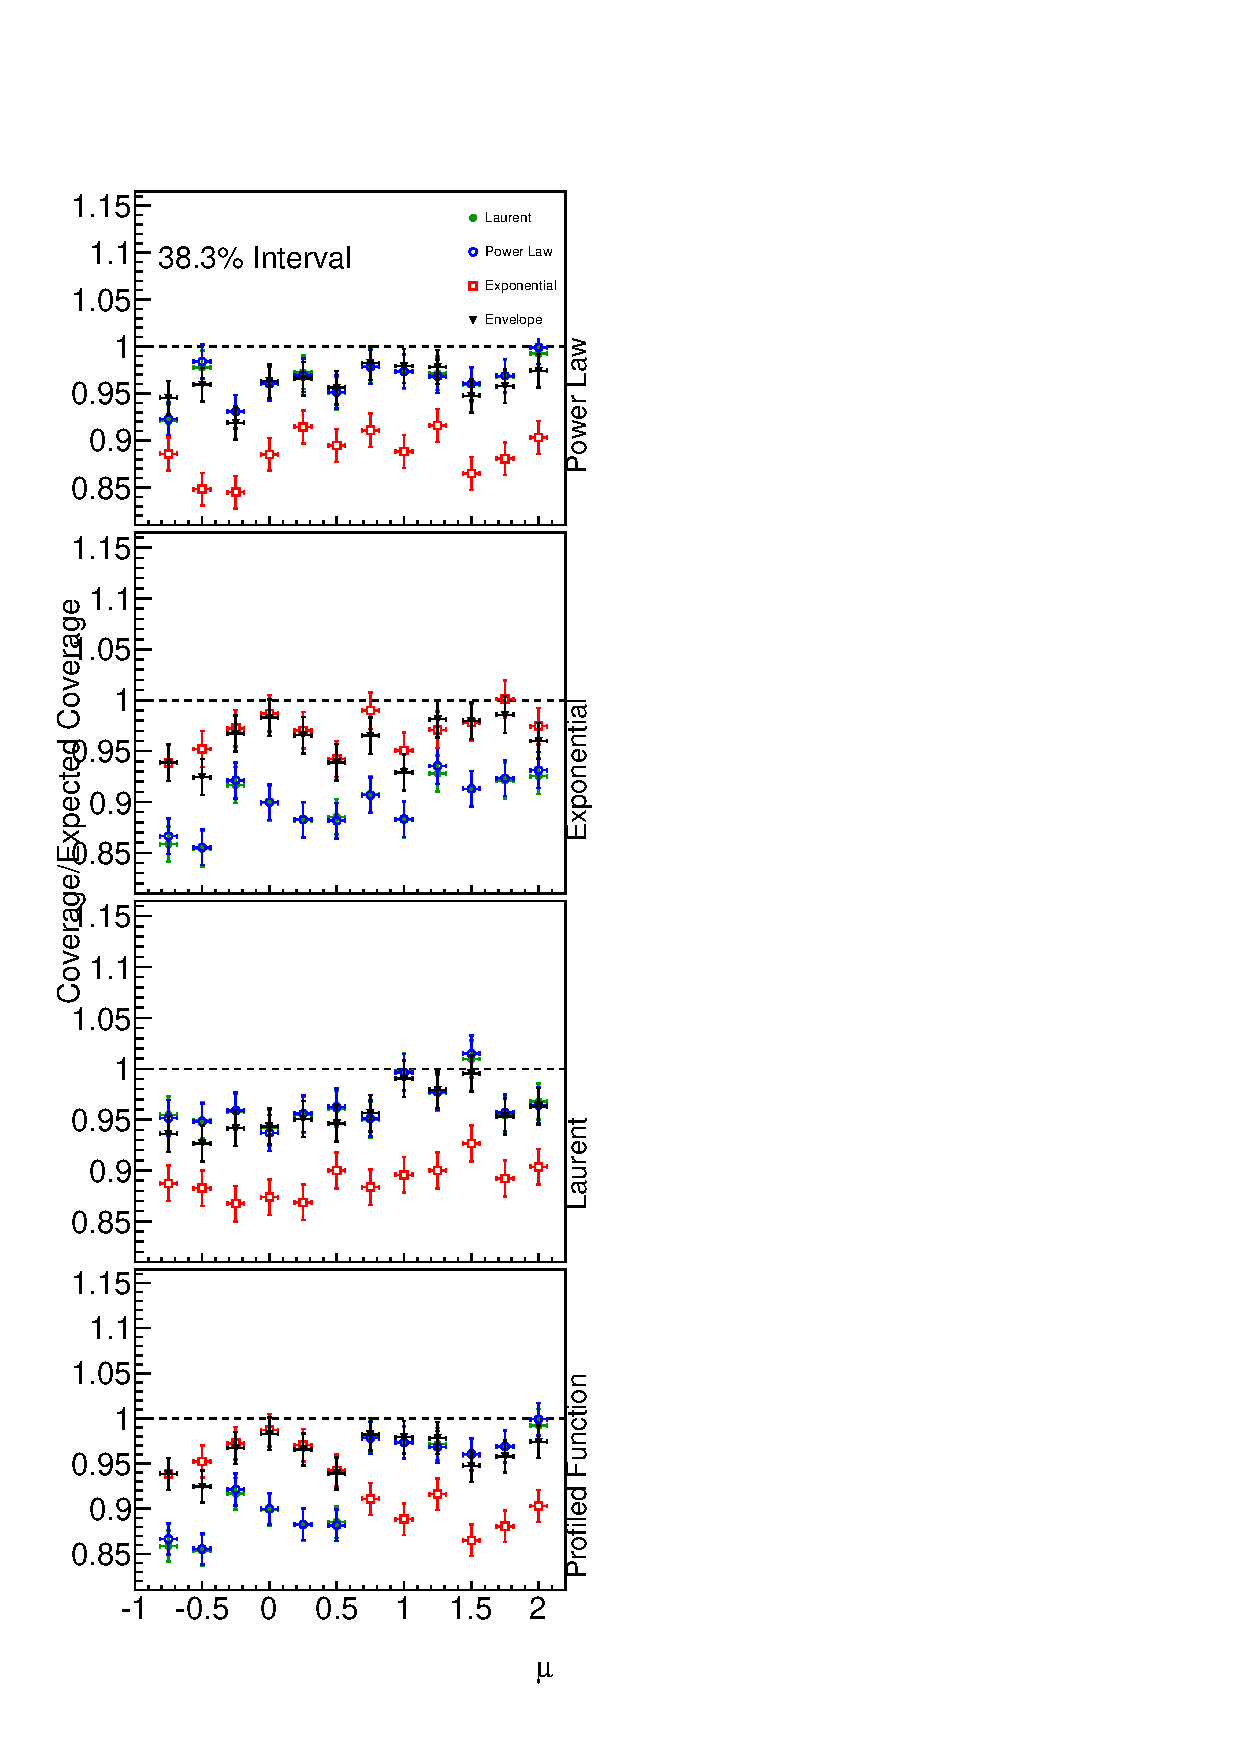
\includegraphics[width=0.45\textwidth]{{functions/FirstOrderFunctions_Coverage_0.5}.pdf}
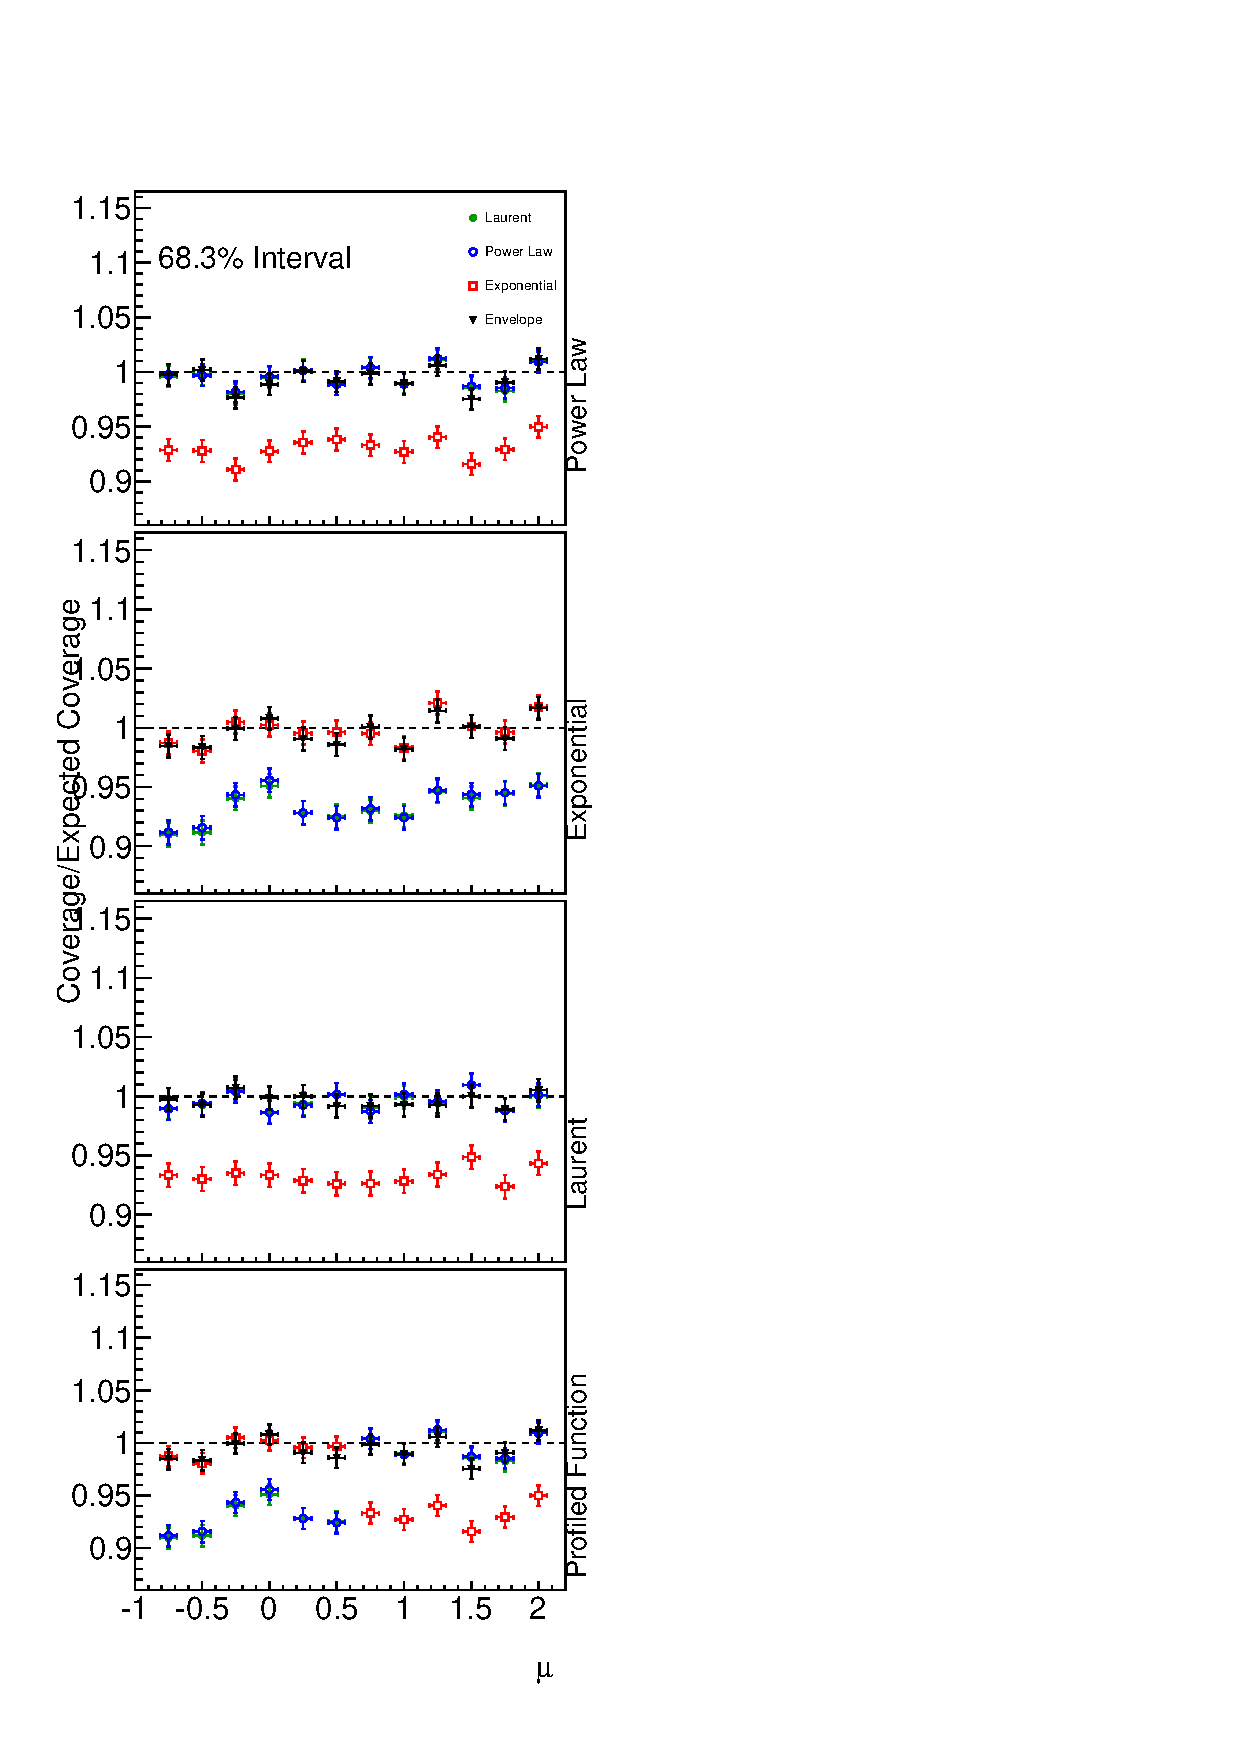
\includegraphics[width=0.45\textwidth]{{functions/FirstOrderFunctions_Coverage_1.}.pdf}\\
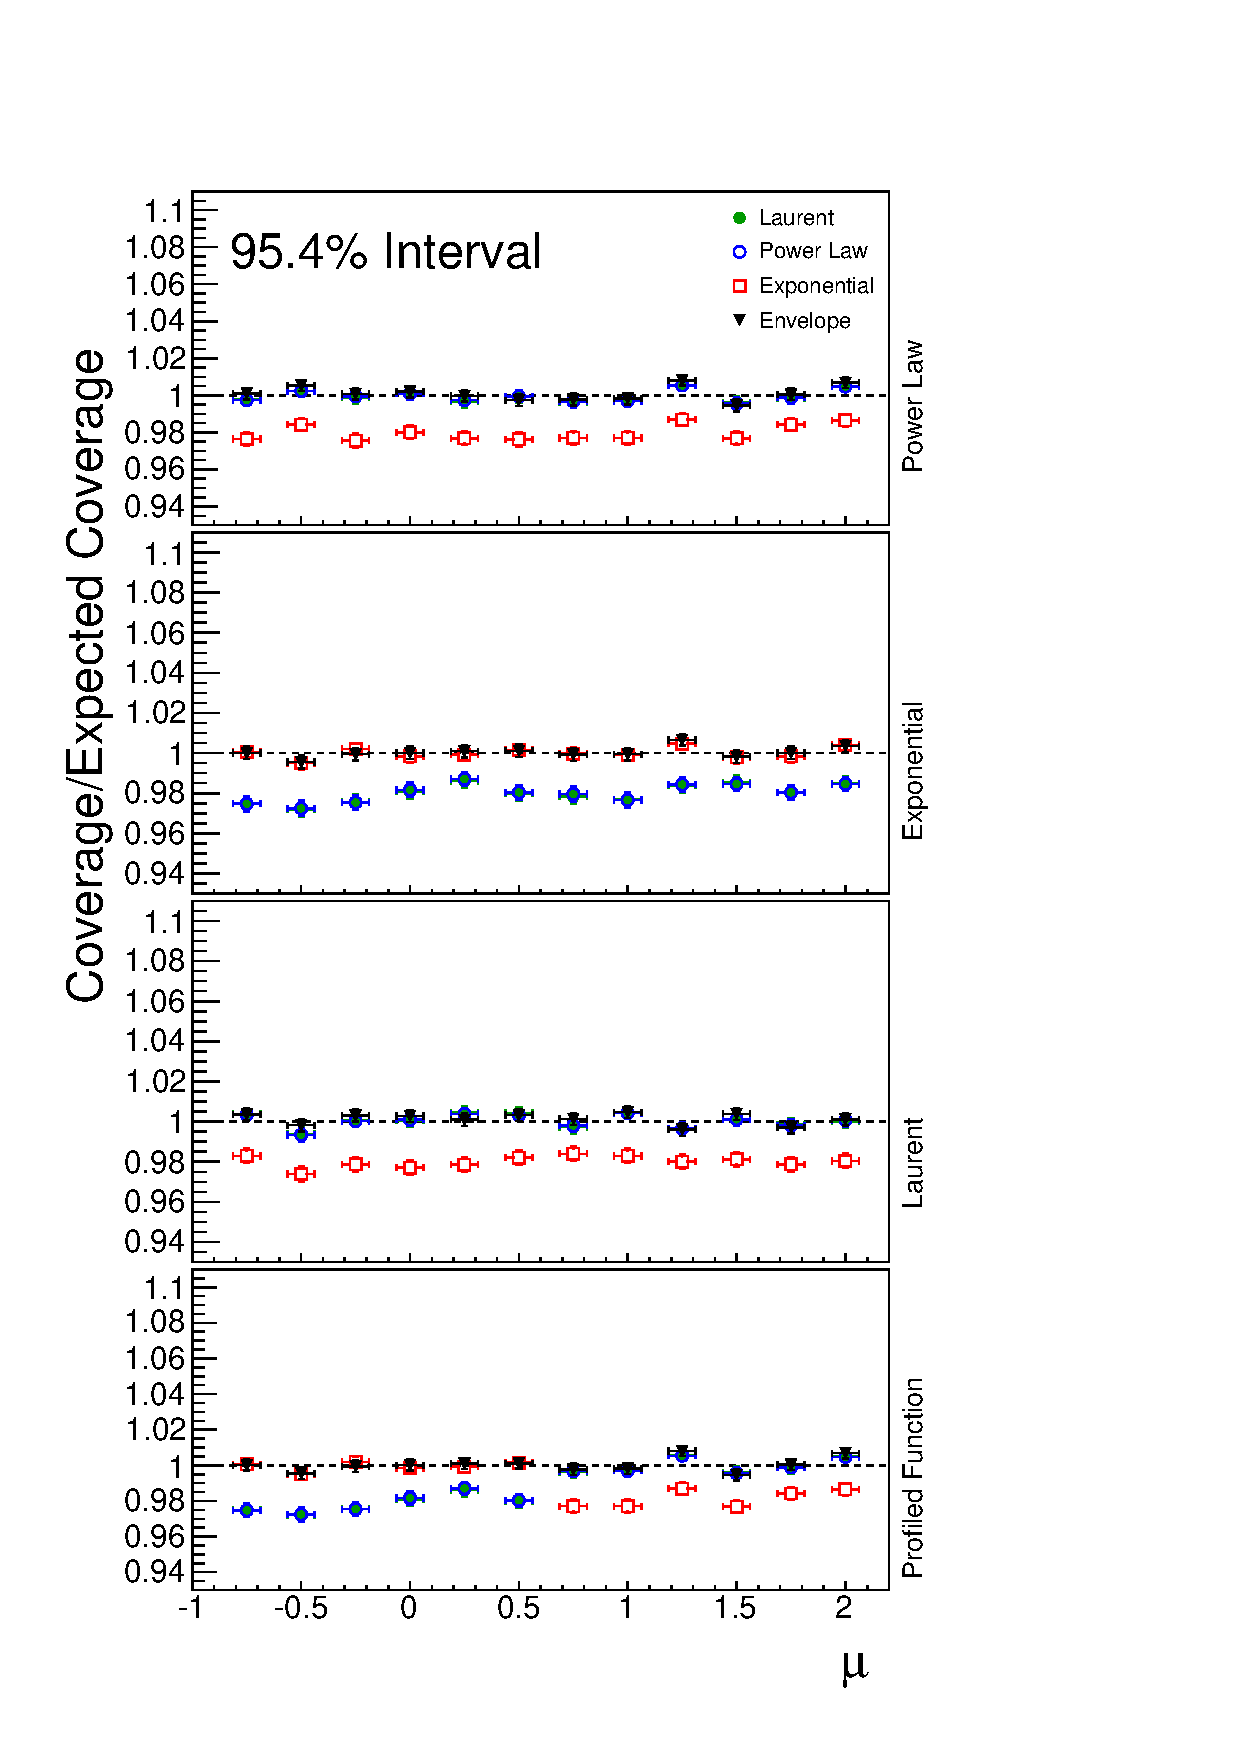
\includegraphics[width=0.45\textwidth]{{functions/FirstOrderFunctions_Coverage_2.}.pdf}
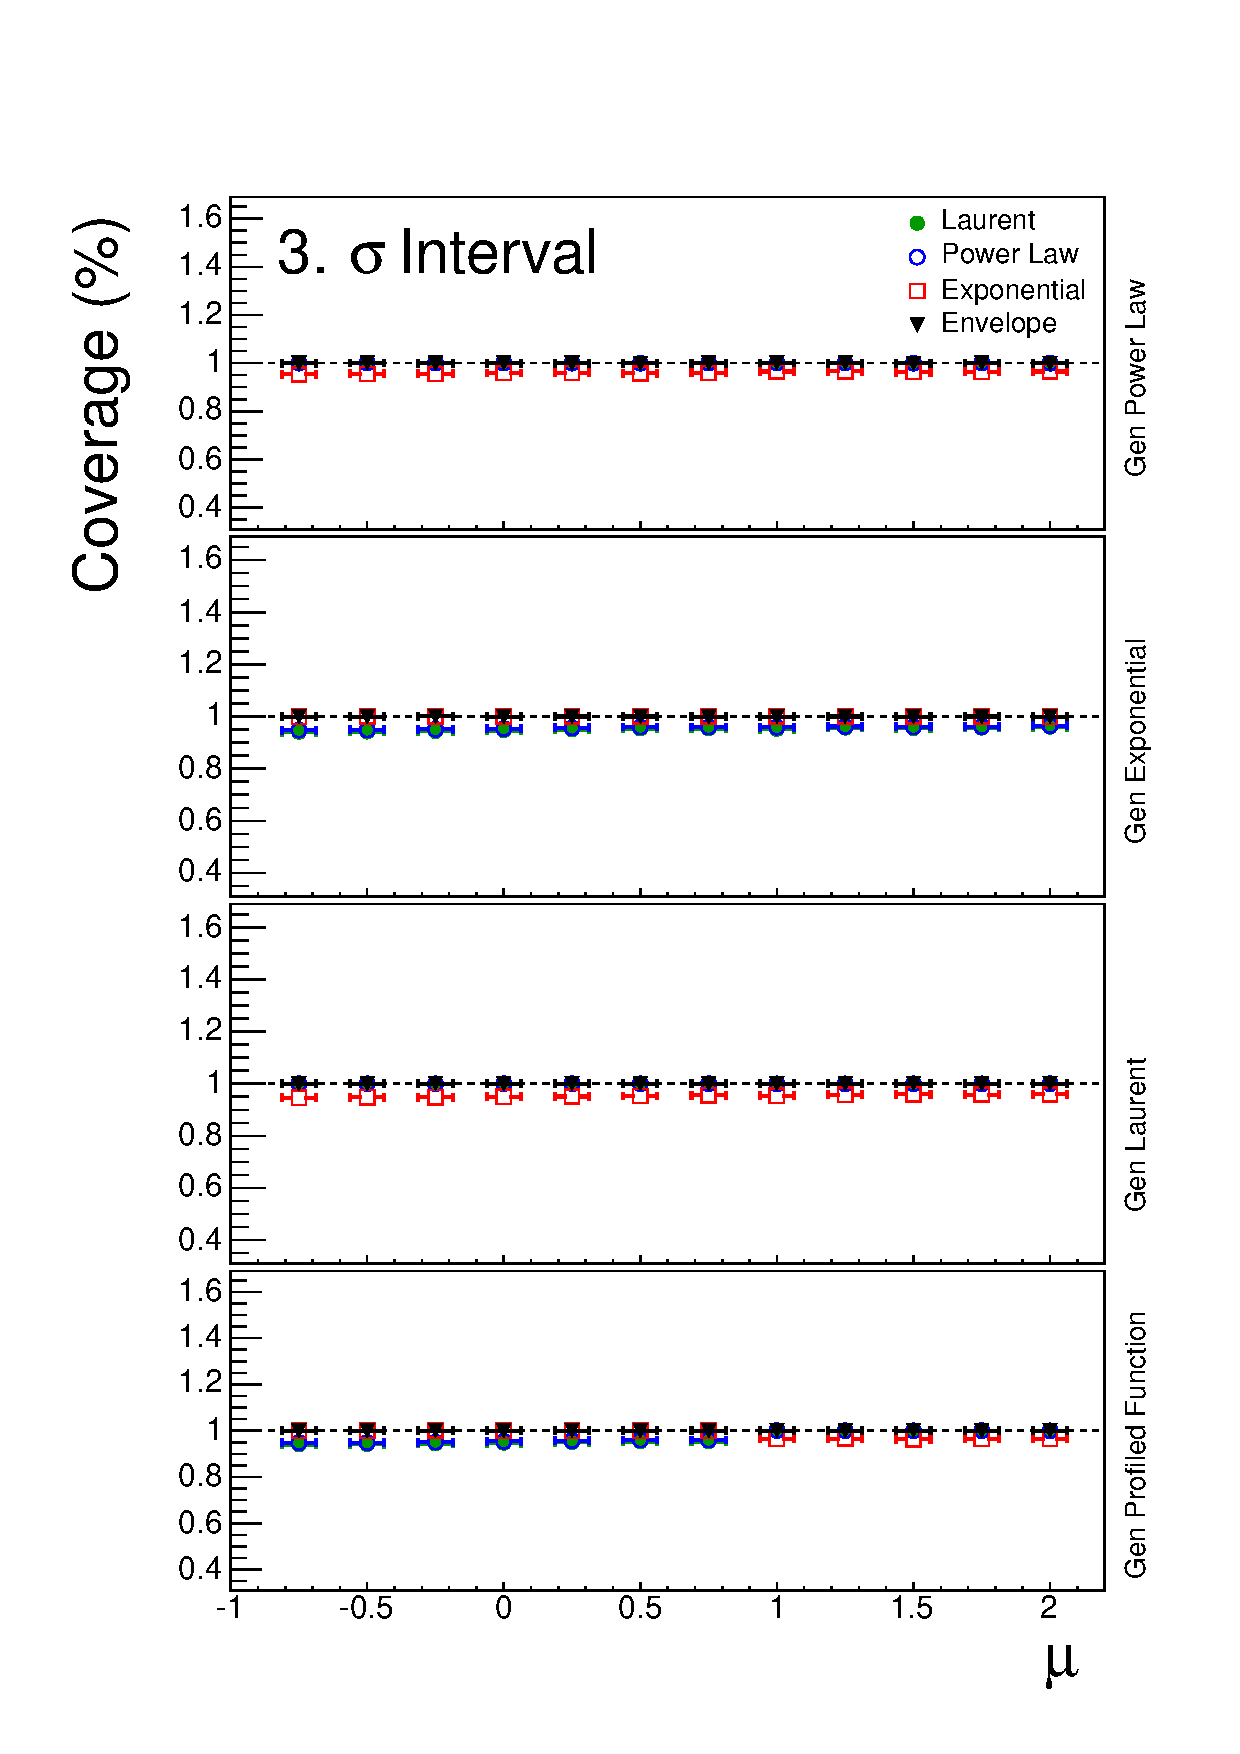
\includegraphics[width=0.45\textwidth]{{functions/FirstOrderFunctions_Coverage_3.}.pdf}
\caption{Fraction of toys in which the fitted value of $\mu$ is within the 38.3\%, 68.3\%, 95.4\% and
99.7\% intervals relative to the expected fraction for that interval using a single
function and using the envelope.
Within each subfigure,
the first, second and third plots shows the results
when the generating background function is the power law, exponential and Laurent,
respectively. The last plot in each subfigure
shows the result when the best-fit function at each
value of $\mu$ is used to generate toys. Within each panel the different
points correspond to a different fitting function: Laurent (solid green), power law (open blue), exponential (open red) and the envelope of all four two-parameter functions (solid black). In all cases,
fitting with the polynomial gives values outside the range of these plots.}
\label{fig:functions:firstordercoverage}
\end{figure}


%ASIMOV RESULTS AS PART OF DISCUSSION ON BIAS?

%UNBINNED MENTIONED ONLY IN PASSING


%\subsection{Toy generation}
%\label{sec:functions:toys}

%WHAT IS A BETTER TERM THAN ``TOYS''?

%1. USING SINGLE FUNCTION (GIVING BIAS)

%2. USING BAYESIAN PROBABILITY MIX OF FUNCTIONS (NO BIAS)

%3. USING FREQUENTIST FRACTIONAL CONTRIBUTIONS OF FUNCTIONS (BIAS???)
